\section{Descripción General}
En este documento se desarrollarán las motivaciones, implicaciones y detalles de la implementación de este Trabajo de Fin de Grado.

El objetivo general de este proyecto ha sido el desarrollo de un videojuego educativo en conjunto con otra alumna, \nombrecoautorespacio que se ha encargado de la del diseño y el arte del videojuego.
Este videojuego tiene como meta servir como apoyo para el desarrollo del Pensamiento Computacional (en adelante PC) en niños de Primaria/ESO. El PC se define como una habilidad cognitiva que permite resolver problemas
 utilizando estrategias computacionales\cite{tesismaria}, de las cuales se pueden extraer seis factores y sus definiciones\cite{tesismaria}:
\begin{compactitem}
    \item Abstracción: Proceso de obtener algo simple desde algo complejo, obviando los detalles.
    \item Análisis de datos: Buscar, seleccionar, organizar y analizar lógicamente los datos. 
    \item Descomposición de problemas: Descomponer problemas en otros más pequeños que pueden resolverse con mayor facilidad. 
    \item Algoritmia: Identificar instrucciones específicas y explícitas que, paso a paso, llevan acabo un proceso.
    \item Depuración de errores: Identificar y corregir los errores en la solución aportada.
    \item Generalización: Transferir un proceso de resolución de problemas a una variedad grande de problemas.
\end{compactitem}

Partiendo de esta base, se ha desarrollado el videojuego EcoRescue con el objetivo de añadir elementos jugables que ayuden a potenciar gran parte de todas estas facetas del PC. Dado que este proyecto se ha desarrollado en conjunto con otra alumna, la documentación del diseño queda fuera del alcance de este documento, sin embargo, sí que habrá referencias al Game Design Document (GDD) cuando sea preciso para ilustrar el punto que se esté desarrollando en ese momento.

EcoRescue es un videojuego que además de ser un apoyo en el desarrollo del PC, pretende ser didáctico con los temas que muestra y enseñar a los niños que lo jueguen información acerca del medio ambiente y la restauración de ecosistemas, siendo así la mecánica principal restaurar los ecosistemas en los que consisten sus niveles. Con este fin se ha contado con el apoyo de la Doctoranda en restauración de ecosistemas, \nombreproductor.

Las mecánicas de EcoRescue se pueden definir en dos fases, la de investigación y la de restauración. Al iniciar el juego, el jugador se encuentra con una lista de niveles que muestran una serie de biomas y características a restaurar, una vez entra, comenzará la fase de investigación:
\begin{compactitem}
    \item Durante la fase de investigación, el jugador puede observar un mapa cuadriculado en vista isométrica con varios biomas visibles.
    \item Encima de cada bioma, verá una burbuja con un icono (Figura \ref{fig:burbujas}) con la que deberá interactuar para aprender sobre qué le puede estar ocurriendo al bioma.
    \item Esta interacción muestra un libro con información acerca del bioma, su alteración y sus problemas (Figura \ref{fig:libro}).
    \item El jugador tendrá que completar un minijuego en el que relacione los problemas con sus posibles consecuencias (Figura \ref{fig:relations}) para demostrar que ha entendido qué es lo que le está ocurriendo al bioma.
\end{compactitem}

\begin{figure}[H]
  \centering
	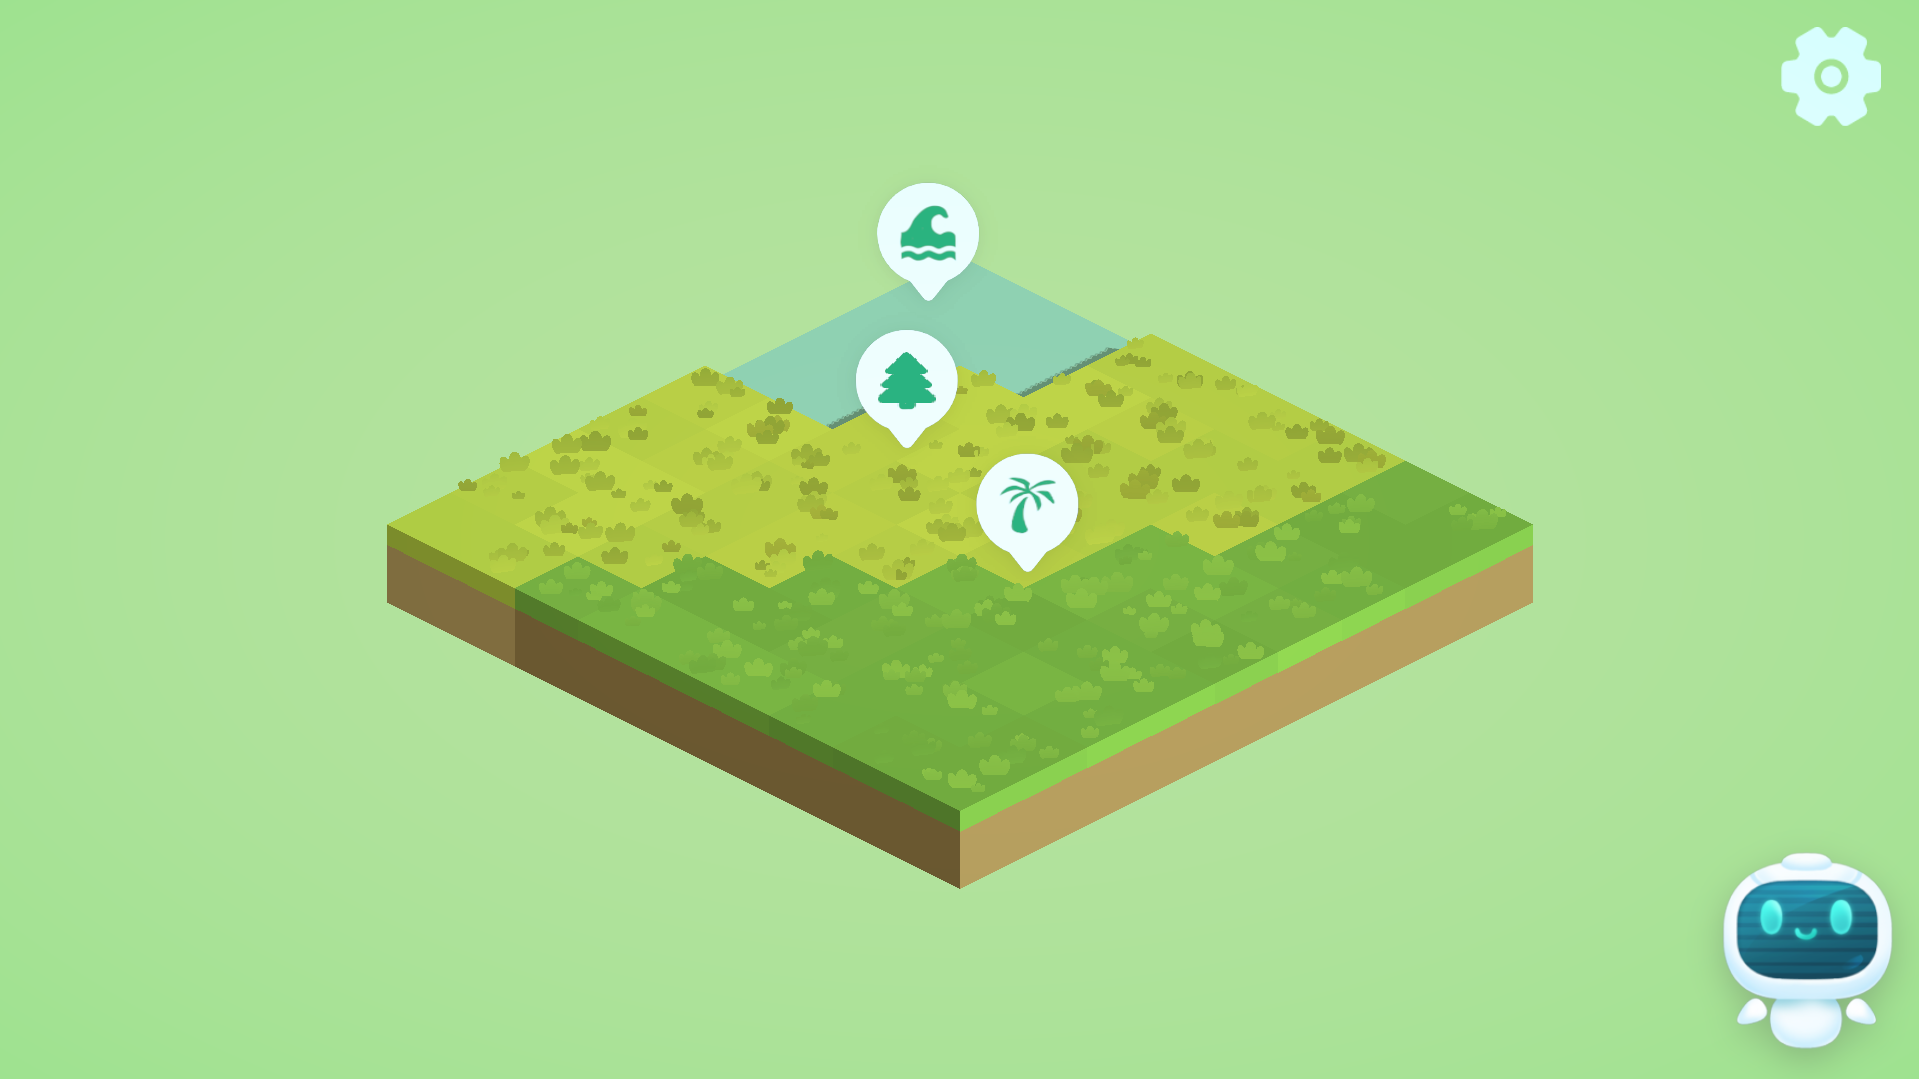
\includegraphics[width=350px,clip=true]{burbujas.png}
  \caption{Mapa con burbujas de bioma visibles}
  \label{fig:burbujas}
\end{figure}

\begin{figure}[H]
  \centering
	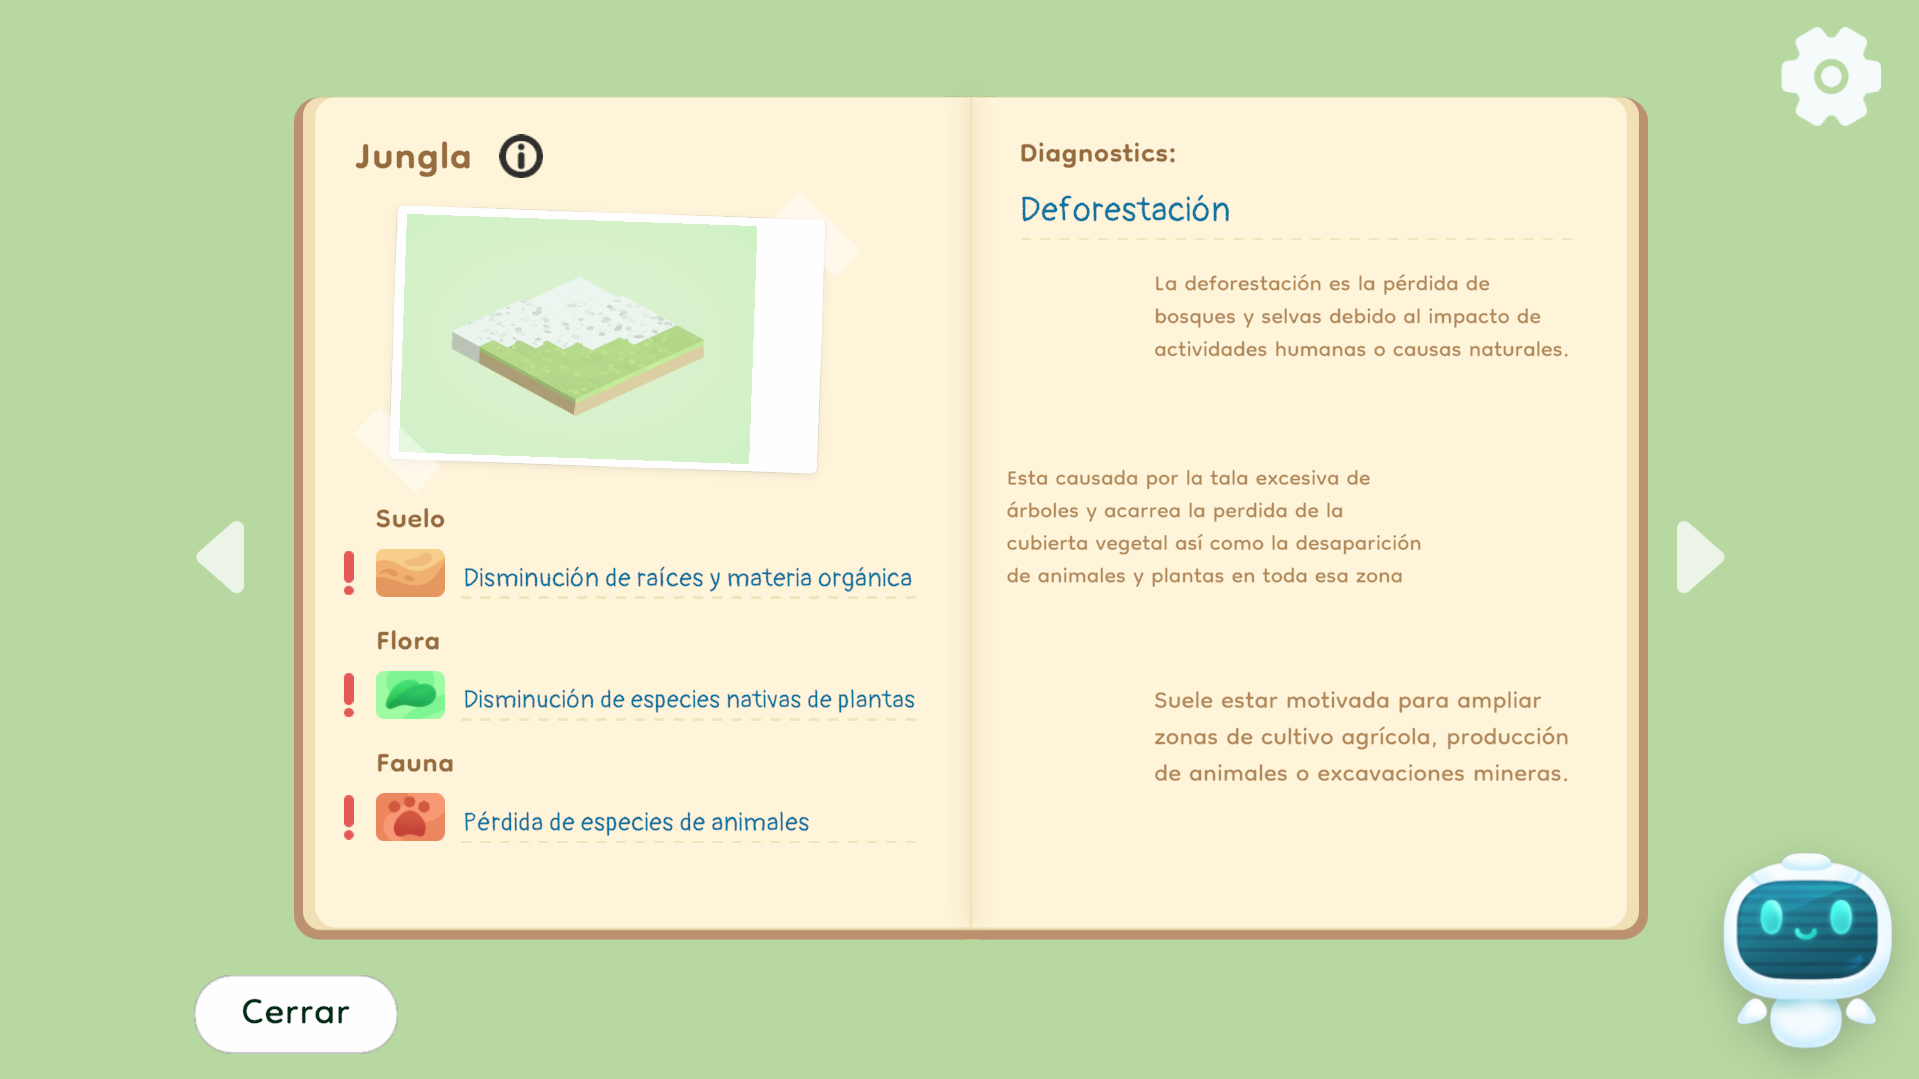
\includegraphics[width=350px,clip=true]{libro_info.png}
  \caption{Libro con información de problemas medioambientales}
  \label{fig:libro}
\end{figure}

\begin{figure}[H]
  \centering
	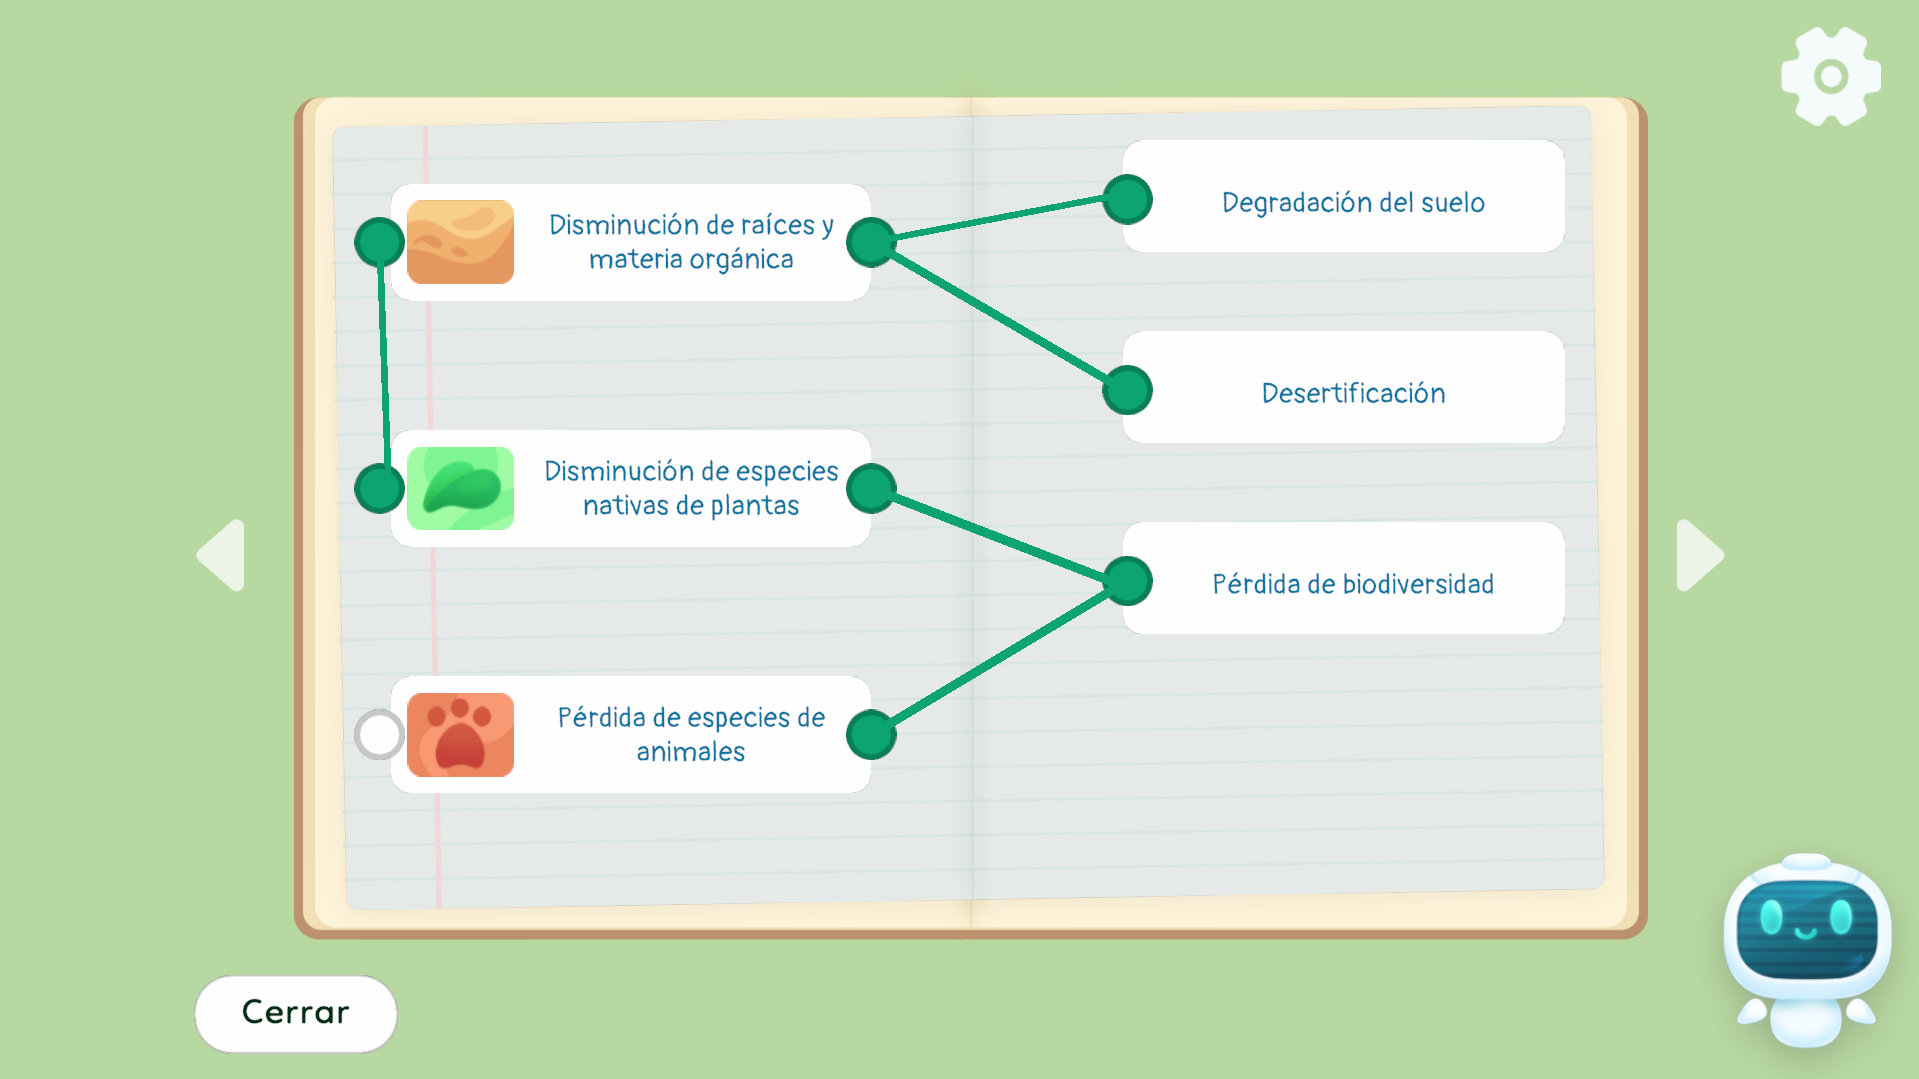
\includegraphics[width=350px,clip=true]{libro_relaciones.png}
  \caption{Libro de Relaciones Problema - Consecuencia}
  \label{fig:relations}
\end{figure}

Una vez el jugador haya demostrado que ha entendido todas las alteraciones y problemas de todos los biomas, el juego pasará a la segunda fase, la de restauración.
\begin{compactitem}
    \item Durante la fase de restauración, el jugador tendrá un presupuesto de energía para gastar en máquinas restauradoras.
    \item Cada bioma tendrá una alteración, que a su vez estará compuesta de 2-3 fases, cada una definida por un problema distinto (Deforestación, Desertificación, Sobrepesca…)
    \item El jugador deberá comprar máquinas restauradoras de la tienda y colocarlas en el bioma para que puedan hacer efecto, los distintos efectos de estas restaurarán el ecosistema de una forma u otra.
    \item La jugabilidad radica en que el jugador tendrá distintas opciones de máquinas (tres) por cada fase de cada bioma, y cada opción tendrá un efecto distinto, teniendo en cuenta la información que ha adquirido durante la primera fase, y la información que proporciona la tienda acerca del efecto de la máquina, el jugador deberá hacer una elección que le permita restaurar el ecosistema por un coste apropiado, con el objetivo de no quedarse sin presupuesto antes de terminar todas las fases de todos los biomas.
\end{compactitem}

Teniendo en cuenta las estrategias del PC y las mecánicas del juego, podemos asimismo definir una tabla (Tabla \ref{fig:tablaPCMecanicas}) que las relacione entre sí, dejando claro de qué forma se pretende ayudar a potenciar el PC en los jugadores.
\raggedbottom
\begin{table}[H]
\begin{center}
\setlength{\tabcolsep}{5pt}
\renewcommand{\arraystretch}{1.2}
\begin{tabular}{ | m{8em} | m{30em} | } 
  \hline
  Estrategia & Mecánica \\ 
  \hline
  Abstracción & A la hora de realizar los diagramas de correlación entre indicadores (datos) y sus consecuencias, se reduce al mínimo imprescindible la explicación del contexto de la alteración del ecosistema. \\ 
  \hline
  Análisis de Datos & La fase de investigación muestra una serie de datos que posteriormente el jugador analiza para poder correlacionarlos con consecuencias. \\ 
  \hline
  Descomposición de problemas & Un nivel está visiblemente desglosado en diferentes tareas y subtareas. Para completar el nivel es necesario restaurar todos los biomas y para restaurar cada bioma hay que finalizar todas las fases del plan de restauración (que pueden considerarse tareas a cumplimentar). \\ 
  \hline
  Algoritmia & A la hora de restaurar un ecosistema, está todo claramente separado de forma secuencial. Incluso el propio nivel se desarrolla de forma secuencial. \\ 
  \hline
  Depuración de Errores & Es posible cometer errores y es importante detectarlos y subsanarlos a tiempo. La idea es dejar cierto margen para que los jugadores puedan echarse atrás y arreglar los fallos. \\ 
  \hline
    & El jugador tiene recursos (moneda) limitados y debe hacer un buen uso de ellos para poder completar los niveles, si se queda sin dinero, deberá volver a intentarlo para poder minimizar el gasto. \\ 
  \hline
  Generalización & A menudo las alteraciones de los ecosistemas tienen factores en común, a lo largo del progreso en el videojuego los jugadores podrán ir discerniendo que existen muchas correlaciones entre alteraciones y sus consecuencias. Por ejemplo: Si hay un problema con el suelo (del tipo que sea) la flora no va a poder prosperar correctamente y si la flora no está en sus condiciones óptimas, la fauna tampoco lo estará. \\ 
  \hline
\end{tabular}
\centering
\caption{Relaciones entre Estrategias del PC con mecánicas del videojuego.}
\label{fig:tablaPCMecanicas}
\end{center}
\end{table}

\section{Motivación}

La motivación para el desarrollo de EcoRescue nace como respuesta al Plan de Acción de Educación Digital 2021-2027 de la Comisión Europea\cite{europaPlan}, además de verse reforzada en 
España por la modificación de la Ley Orgánica 3/2020 del 3 de diciembre de 2020\cite{lomce}, y los Reales Decretos 95/2022\cite{boeInfantil}, 157/2022\cite{boePrimaria}, 217/2022\cite{boeSecundaria} y 243/2022\cite{boebachillerato}, del 1 de febrero, 1 y 19 de marzo y 5 de abril del 2022 respectivamente, 
que establecen las enseñanzas mínimas de la educación, incluyendo el PC, en las etapas de Educación Infantil, Primaria y Secundaria Obligatoria y Bachillerato, como una competencia transversal en diversas asignaturas o en asignaturas determinadas.

Como se ha mencionado anteriormente, además de servir para desarrollar el PC, uno de los objetivos del proyecto es concienciar sobre la importancia de cuidar el medioambiente y de como distintos indicadores y alteraciones pueden afectar negativamente a estos. De esta forma, el juego puede ayudar a niños y adolescentes a relacionar consecuencias del sistema productivo de la sociedad actual con los daños que sufren actualmente nuestros ecosistemas y entornos naturales. A su vez, ilustra de forma eficiente como interaccionan diferentes ecosistemas entre sí y como se relacionan sus diferentes elementos: fauna, flora y el soporte natural. Además, el juego aporta una versión optimista de como entornos que se consideran destruidos se pueden recuperar mediante la intervención y tecnología adecuados. 

Este enfoque es relevante dado que según los Reales Decretos mencionados anteriormente\cite{boeInfantil}\cite{boePrimaria}\cite{boeSecundaria}\cite{boebachillerato} se estipula que en lo relacionado al Conocimiento del Medio, Biología y Geología se buscará fomentar el razonamiento y pensamiento crítico (computacional) para resolver problemas o dar explicación a procesos de la vida cotidiana.

Finalmente habría que considerar también la motivación adicional de aprender el uso de nuevas tecnologías mediante el desarrollo de un proyecto, que tendría como objetivo el propio aprendizaje y la acumulación de experiencia de llevar un proyecto desde su etapa de concepción hasta validarlo con un grupo de alumnos de instituto.

\raggedbottom
\section{Objetivos}
\subsection{Objetivos generales}
El objetivo general del trabajo es la elaboración de un prototipo funcional del videojuego EcoRescue para el desarrollo del PC y la concienciación en la restauración de ecosistemas, 
en el que los jugadores puedan acceder a niveles generados procedimentalmente, compuestos por un número
de 1-N biomas. Posteriormente deberán poder informarse de estos, relacionar problemas y consecuencias (Figura \ref{fig:diagconsecuencias}) y finalmente 
colocar máquinas en los biomas para restaurar los distintos problemas de cada alteracion.

\begin{figure}[H]
  \centering
    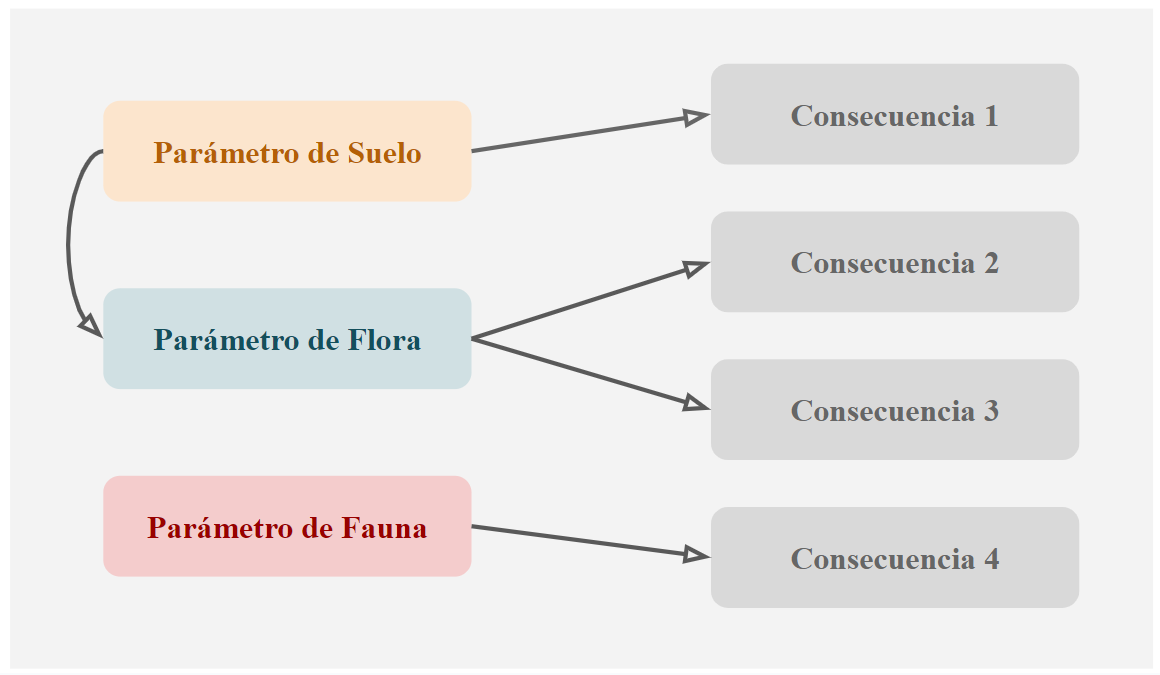
\includegraphics[width=350px,clip=true]{diagramaproblemasconsecuencias.png}
  \caption{Diagrama de relaciones entre problemas y problemas y consecuencias}
  \label{fig:diagconsecuencias}
\end{figure}

El prototipo deberá tener interfaces funcionales que muestren la información de los niveles, biomas, alteraciones, problemas, consecuencias, máquinas y tutoriales (Figuras \ref{fig:UI} y \ref{fig:diagUI}). Los tutoriales vendrán dados por diálogos que saldrán del 
icono de un robot (Figura \ref{fig:robot}) que guiará al jugador durante su experiencia de juego.

\begin{figure}[H]
    \centering
      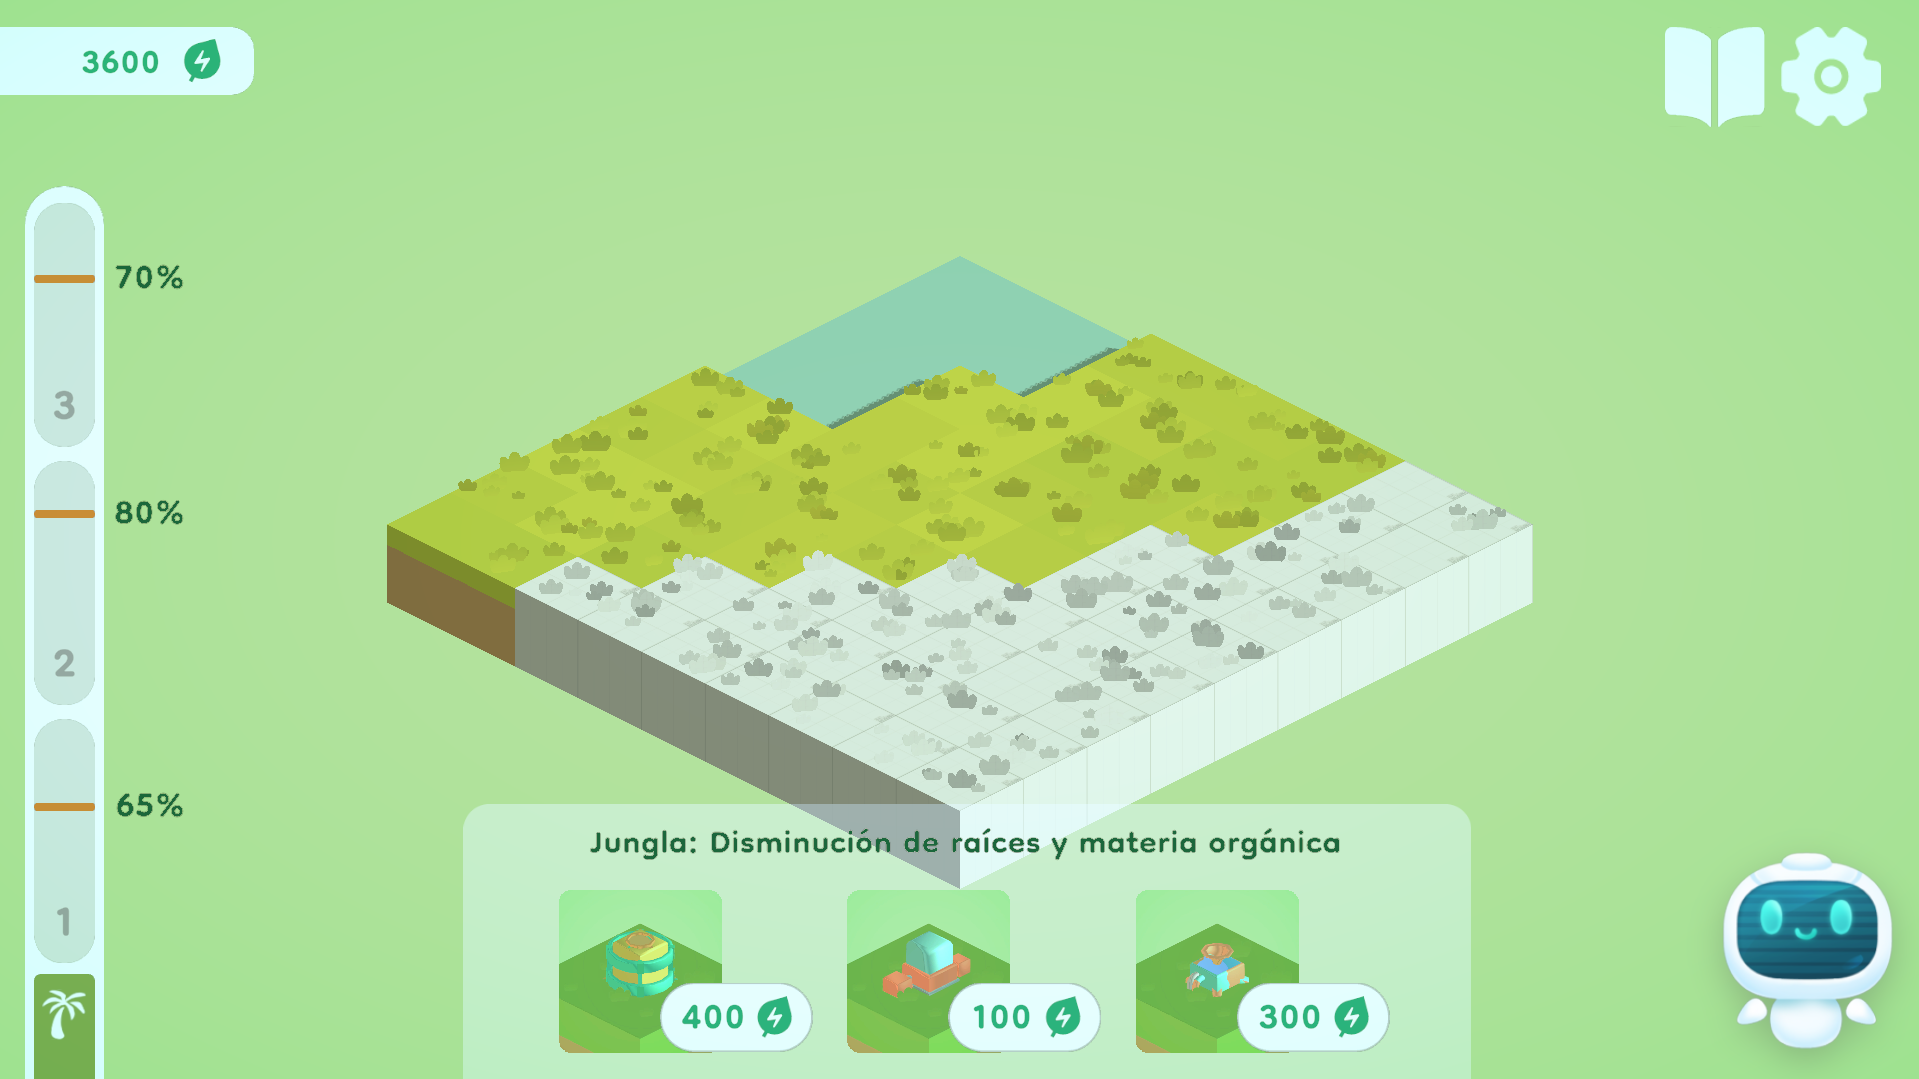
\includegraphics[width=350px,clip=true]{interfaz_restauracion.png}
    \caption{Interfaz general de EcoRescue}
    \label{fig:UI}
\end{figure}

\begin{figure}[H]
    \centering
      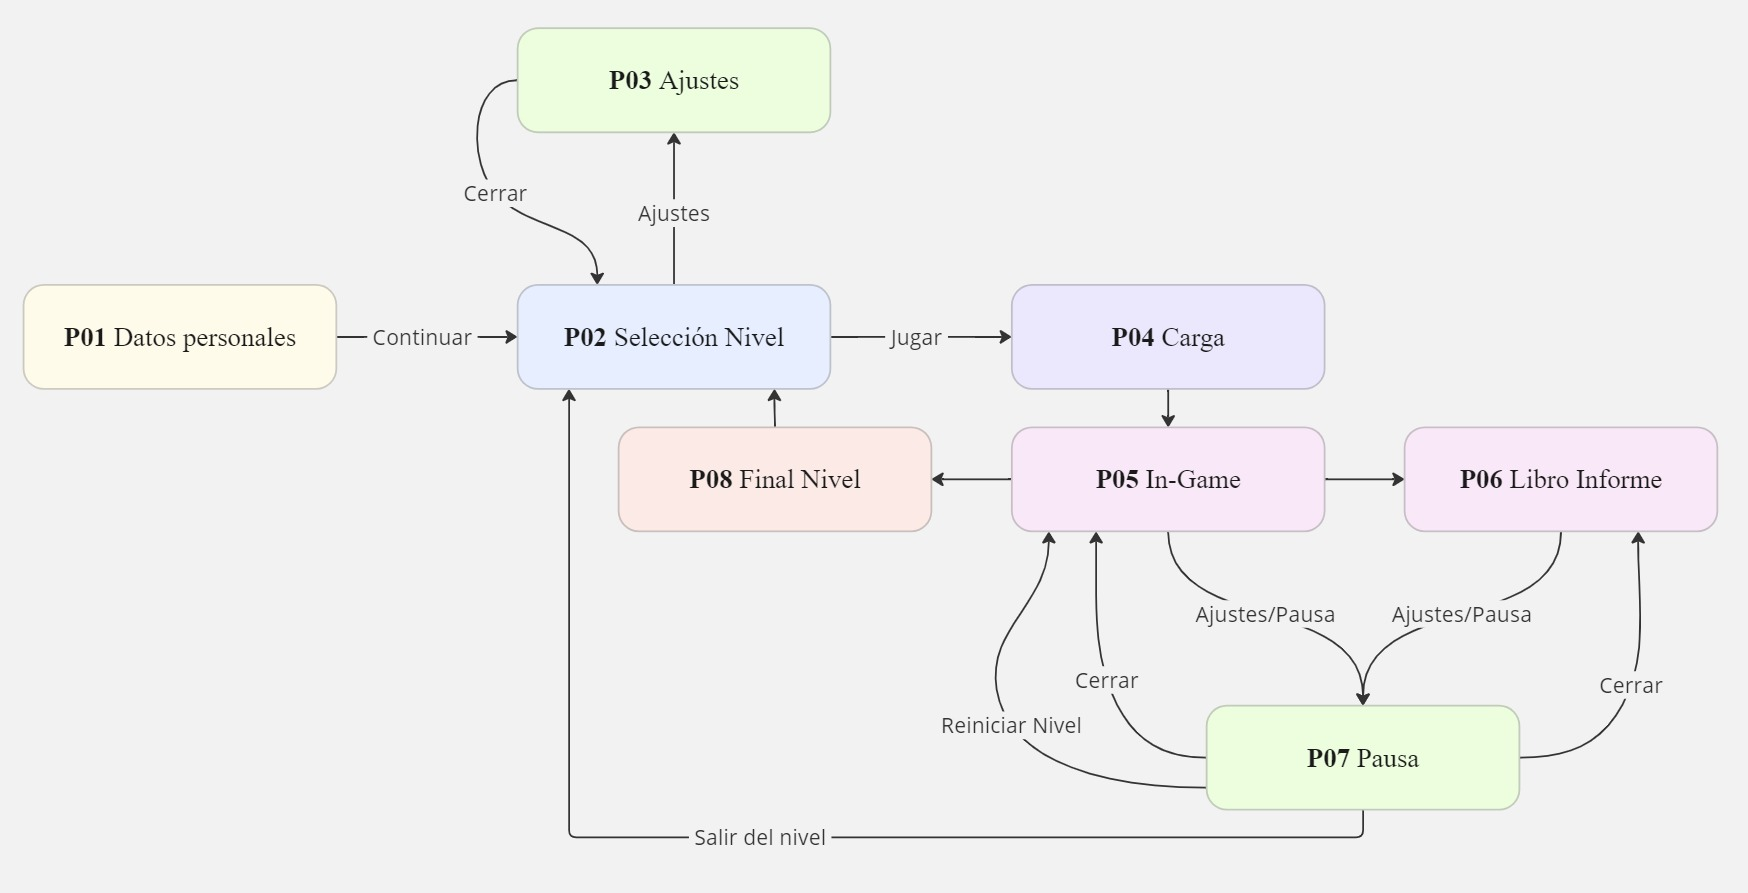
\includegraphics[width=350px,clip=true]{diagramapantallas.jpg}
    \caption{Diagrama de flujo de UI de EcoRescue}
    \label{fig:diagUI}
\end{figure}

\begin{figure}[H]
    \centering
      
\includegraphics[width=350px,clip=true]{convo_robot.png}
    \caption{Conversación de tutorial del robot}
    \label{fig:robot}
\end{figure}

El prototipo también deberá ser jugablemente disfrutable, esto implica desarrollar sistemas de control, sonido y animaciones que hagan que el juego sea vistoso y satisfactorio de jugar.

\subsection{Generación procedimental}

Una parte importante de EcoRescue es la facilidad de creación de contenido, para que desarrollar niveles sea más sencillo, el juego se ha enfocado desde un principio con la generación procedimental en mente, de forma que los niveles deberán generarse en base a algoritmia\cite{FastNoiseLite}, y cosas como las alteraciones en un nivel o el percentil (Figura \ref{fig:percentil}) al que se debe completar una fase deberán del mismo modo seguir un patrón procedimental.

\begin{figure}[H]
  \centering
    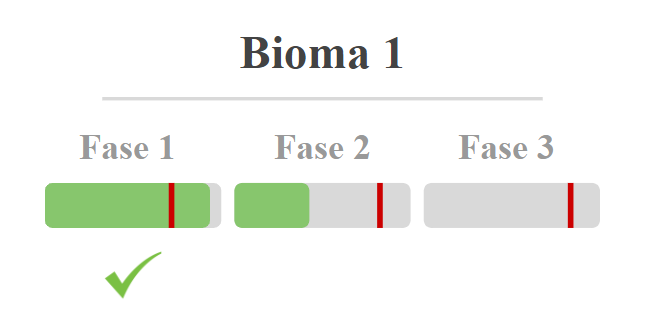
\includegraphics[width=350px,clip=true]{diagramafases.png}
  \caption{Diagrama explicativo de los percentiles a completar de cada fase}
  \label{fig:percentil}
\end{figure}

\subsection{Herramientas del desarrollo}

De cara a la generación procedimental de niveles, el prototipo necesitará herramientas para que enlazar el gran volumen de contenido requerido por este enfoque de desarrollo con las estructuras internas del videojuego sea sencillo y mayormente automatizado. 

De esta forma, se requiere desarrollar un script que importe automáticamente todo el contenido (biomas, alteraciones, problemas, consecuencias, sprites, modelos...) desde un fichero de excel a un formato legible por el juego.

Además, también se requiere la creación de herramientas que permitan elegir de qué forma se quiere que se presente un nivel, incluyendo: personalización de las reglas de la generación procedimental de mapas, selección de Biomas por nivel y selección de Alteraciones por Bioma.

Además, el prototipo necesitará un sistema de generación de diálogos para que el robot de los tutoriales pueda comunicarse efectivamente con el jugador.

\subsection{Recogida de datos}

De cara a la medición de resultados, es necesario que el prototipo sea capaz de comunicarse con una base de datos para poder monitorizar las partidas de los jugadores y así poder interpretar sus movimientos. 
Esta comunicación con la base de datos debería recoger los datos básicos del usuario (nombre, edad...) (Figura \ref{fig:datos}) así como datos sobre su partida (máquinas colocadas, relaciones correctas, veces que ha perdido el nivel...).

\begin{figure}[H]
    \centering
      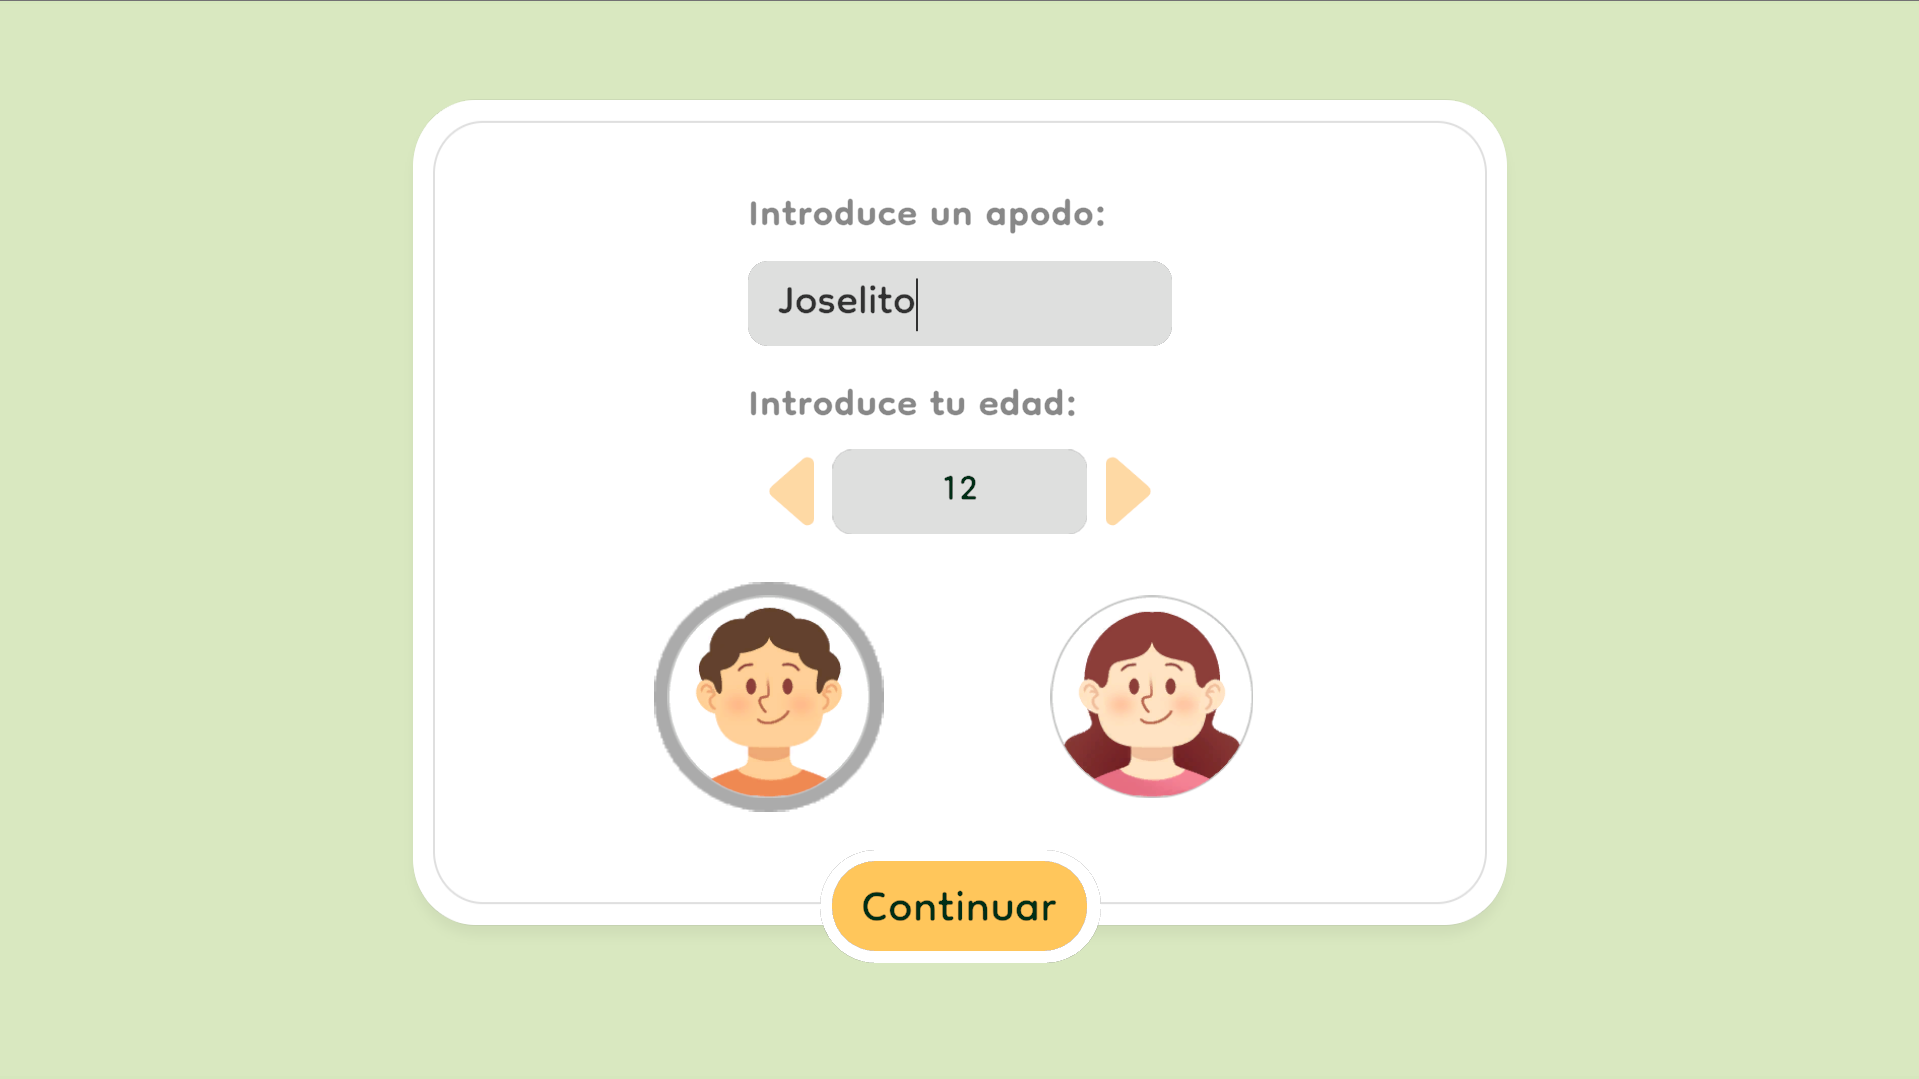
\includegraphics[width=350px,clip=true]{datos_pj.png}
    \caption{Pantalla de introducción de datos personales}
    \label{fig:datos}
\end{figure}

\subsection{Validación}

El objetivo más importante a nivel de proyecto es validar el prototipo frente a un grupo de alumnos de 1º de la ESO reales, con el objetivo de poder utilizar los datos de una encuesta así como los datos obtenidos en la base de datos para poder extraer conclusiones acerca de la efectividad del prototipo como herramienta didáctica para el desarrollo del PC, además de como herramienta divulgativa en lo referente a la restauración de ecosistemas.
Queda patente, pues, que los objetivos de la validación deben ser:
\begin{compactitem}
    \item Que el juego verdaderamente sirva para desarrolar el PC.
    \item Que el juego divulge información interesante acerca de la restauración de ecosistemas.
    \item Que el juego resulte una expriencia amena y divertida, a fin de que los alumnos disfruten del aprendizaje.
\end{compactitem} 

\subsection{Resumen de Objetivos}

En resumen, el el proyecto pretende, como objetivo principal desarrollar un juego completo y funcional que permita al jugador informarse sobre la restauración de ecosistemas y actuar en consecuencia.

Además de los objetivos secundarios:
\begin{compactitem}
  \item Desarrollar el PC del jugador en el aula.
  \item Desarrollar un juego que sea divertido y ameno.
  \item Desarrollar un juego con niveles generados procedimentalmente, además de herramientas que permitan crear contenido de forma eficiente para este.
  \item Recabar información sobre las partidas de los jugadores con el objetivo de interpretar sus movimientos y extraer conclusiones sobre la efectividad del prototipo.
\end{compactitem}

\section{Metodología}

Para el desarrollo del prototipo se ha utilizado una metodología de trabajo iterativa-incremental enfocada en la revisión de objetivos y
avances entre el tutor y los alumnos. Durante una serie de revisiones se ha evaluado el estado del proyecto y se han marcado objetivos de cara a las siguientes revisiones. El desarrollo se puede dividir en tres fases: 
\begin{itemize}
	\item Fase 1: Pre-Producción y Análisis de Requisitos, Junio 2023 - Diciembre 2023
	\item Fase 2: Producción, Enero 2024 - Mayo 2024
	\item Fase 3: Polish y Validación, Junio 2024 
\end{itemize}

La primera fase se utilizó como una ventana de tiempo en la que prototipar los controles y la generación procedimental del mapa, además de realizar un análisis de requisitos y un documento de diseño exhaustivo para tener claro qué clase de prototipo realizar. Este documento de diseño se fue iterando con \nombretutor de cara a la producción final.

Durante la segunda fase se realizó el groso de la producción del juego, con el diseño ya fijado, esta fase consistió sobre todo en implementar el bucle de juego general y definir el contenido que iba a estar presente en el juego final.

La tercera y última fase consistió en la creación de herramientas para el desarrollo de contenido/niveles, pulir el juego añadiendo pequeñas animaciones, efectos y sonidos, implementar un sistema de recogida de datos en tiempo real via una base de datos remota y finalmente acudir a un instituto para poder validar el prototipo con alumnos de verdad.

Esta metodología ha acabado siendo todo un exito con este prototipo, ya que ha permitido un avance progresivo donde no ha acabado habiendo esfuerzo malgastado, esto ha permitido que el desarrollo del prototipo haya sido sólido y no se hayan requerido cambios radicales.